\documentclass[aspectratio=169,10pt,fontset=fandol]{ctexbeamer}
\usepackage{amsmath,amssymb,mathtools,bm,mathrsfs}
\usepackage{graphicx,booktabs,array,tabularx,multirow}
\usepackage{tikz,pgfplots,xparse,xstring,mdframed}
\usetikzlibrary{arrows.meta,calc,angles,positioning,shapes.geometric,graphs}
\pgfplotsset{compat=1.18}

\setbeamerfont{normal text}{size=\normalsize}
\setbeamerfont{title}{size=\large}
\setbeamerfont{subtitle}{size=\normalsize}
\setbeamerfont{frametitle}{size=\large}
\setbeamerfont{framesubtitle}{size=\small}
\setbeamerfont{block title}{size=\normalsize}
\setbeamerfont{block body}{size=\normalsize}
\setbeamerfont{section in toc}{size=\normalsize}
\setbeamerfont{section in head/foot}{size=\footnotesize}
\setbeamerfont{author in head/foot}{size=\footnotesize}
\setbeamerfont{title in head/foot}{size=\footnotesize}
\setbeamerfont{date in head/foot}{size=\footnotesize}
\setbeamertemplate{navigation symbols}{}
\setbeamertemplate{itemize item}{\normalsize\textbullet}
\setbeamertemplate{itemize subitem}{\small\textbullet}
\setbeamercolor{structure}{fg=blue!65!black}
\setbeamercolor{block title}{fg=blue!65!black,bg=blue!8}
\setbeamercolor{block body}{fg=black,bg=blue!3}
\setbeamertemplate{footline}{\leavevmode\hbox to\paperwidth{\hfill{\footnotesize\insertframenumber}\hspace*{1em}}\vskip3pt}

% ctex fontset=fandol; system fonts are not redistributed.

\newenvironment{proofdetail}{\par\noindent\textbf{证明：}\quad}{\par}
\renewenvironment{solution}{\par\noindent\textbf{解：}\quad}{\par}
\newenvironment{extra}{\par\textbf{选读}}{\par}
\title{图中文字与长证明.tex}
\begin{document}
\section{微分}
% FRAME-ID F001
\begin{frame}[t,fragile]{目录}
\normalsize
{\color{blue}\normalsize 1. 微分\par}\vspace{0.22em}
\end{frame}
% FRAME-ID F002
\begin{frame}[t,fragile]{微分}
\normalsize
{\normalsize
% PRESENTATION-SCAFFOLD isotropic coordinates; node font size unchanged
\tikzset{every picture/.append style={scale=0.75}}
% SOURCE-BEGIN U0001 0 120
\begin{center}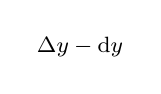
\begin{tikzpicture}
\node at (0,0) {\footnotesize $\Delta y-\mathrm{d}y$};
\end{tikzpicture}\end{center}
% SOURCE-END U0001
}
\end{frame}
% FRAME-ID F003
\begin{frame}[t,fragile]{微分}
\normalsize
{\normalsize
% SOURCE-BEGIN U0002 0 60
\begin{itemize}\item 成本 $C(x)$。\item 收入 $R(x)$。\end{itemize}
% SOURCE-END U0002
}
\end{frame}
% FRAME-ID F004
\begin{frame}[t,fragile]{微分}
\footnotesize
{\footnotesize
% SOURCE-BEGIN U0003 0 114
\begin{extra}\begin{proofdetail}
完整推导步骤。\[a+b=c\]

完整推导步骤。\[a+b=c\]

完整推导步骤。\[a+b=c\]

完整推导步骤。\[a+b=c\]


% SOURCE-END U0003
% PRESENTATION-SCAFFOLD close continued environment
\end{proofdetail}\end{extra}
}
\end{frame}
% FRAME-ID F005
\begin{frame}[t,fragile]{微分（续1）}
\footnotesize
{\footnotesize
% REPEATED-CONTEXT environment continuation
\begin{extra}\begin{proofdetail}

% SOURCE-BEGIN U0003 114 194
完整推导步骤。\[a+b=c\]

完整推导步骤。\[a+b=c\]

完整推导步骤。\[a+b=c\]

完整推导步骤。\[a+b=c\]


% SOURCE-END U0003
% PRESENTATION-SCAFFOLD close continued environment
\end{proofdetail}\end{extra}
}
\end{frame}
% FRAME-ID F006
\begin{frame}[t,fragile]{微分（续2）}
\footnotesize
{\footnotesize
% REPEATED-CONTEXT environment continuation
\begin{extra}\begin{proofdetail}

% SOURCE-BEGIN U0003 194 302
完整推导步骤。\[a+b=c\]

完整推导步骤。\[a+b=c\]

完整推导步骤。\[a+b=c\]

完整推导步骤。\[a+b=c\]

\end{proofdetail}\end{extra}
% SOURCE-END U0003
}
\end{frame}
\end{document}
